\documentclass[Bachelorarbeit.tex]{subfiles}
\begin{document}
\chapter{Evaluation}
\label{chap:evalutation}
Nachdem der Prototyp implementiert wurde, stellt sich die Frage, ob die Entwicklung und Ausarbeitung einen Mehrwert für Anwender\_innen darstellt. 
Dies soll nun mittels der Evaluation geklärt werden.
Für diesen Zweck sowie etwaige Schwachstellen aufzufinden soll der Prototyp im Rahmen einer Usability-Analyse auf Effektivität, Effizienz und Zufriedenstellung \cite[vgl.][Abs.: 3]{Iso9241_11} untersucht werden (siehe Abschnitt: \nameref{Methodik}).
Zusätzlich zu der Usability Analyse soll auch die Art und Weise untersucht werden wie die verschiedenen Ansichten (Karte und Liste) währende des Testes verwendet werden.\\
\\
Der Ablauf der Usability Evaluation sieht dabei wie folgt aus.
Im ersten Schritt werden der Zweck der Analyse sowie die zu untersuchenden Kriterien (siehe Absatz: \nameref{Usability}) erläutert.
Darauf folgt die Festlegung und Beschreibung der Verfahren welche zum Messen der Kriterien angewandt werden.
Basierend auf den definierten Verfahren, wird die Erstellung und Begründung für die Auswahl des Testmaterials dargelegt, welche in der finalen Version auch im Anhang zu finden ist (siehe Anhang: \ref{anhangTestmaterial} - \nameref{anhangTestmaterial}).
Im Abschnitt \nameref{Stichproben} wird der Rahmen für die Tests sowie die Auswahl der Proband\_innen festgelegt.
Die anschließende Dokumentation sowie die Ergebnisse der Durchführung werden im Abschnitt \nameref{Ergebnisse} aufgezeigt.
Abschließend findet eine \nameref{InterpretationDiskussion} auf der Basis der Ergebnisse statt die zum einen die Evaluation der \nameref{Hypothese} sowie den Mehrwert der wählbaren Ansichten  klärt.

\section{Methodik}
\label{Methodik}

Da die Interviews im Vorfeld ergeben haben, dass jede befragte Person einen unterschiedlichen Ablauf sowie unterschiedliche Werkzeuge bei der Planung der Außendienstrouten einsetzt, hilft ein vergleichender Test zwischen Status Quo und Prototyp an dieser Stelle nicht weiter.
Aus diesem Grund liegt es nahe einen klaren Schnitt zu den diversen alten Systemen zu ziehen und eine Formative Usability Evaluation\footnote{Bei der Formativen Evaluation wird anhand definierter Kriterien untersucht ob der Entwurf weiter optimiert werden kann. (vgl. \cite{Burmester}, S. 343)} nach den Kriterien der ISO 9241 durchzuführen.
Dafür soll der Prototyp auf die folgende Hypothesen hin mit Benutzerorientierten Methoden\footnote{Dabei liegt der Fokus bei den Tests auf definierten Anwender\_innen-Gruppen. (vgl. \cite{Burmester}, S. 343)} untersucht werden.


\subsection{Hypothese}
\label{Hypothese}

Der Prototyp unterstützt die potentiellen Pery-Anwender\_innen messbar in den Bereichen Effektivität, Effizienz und Zufriedenstellung bei der Planung von Außendiensteinsätzen (Die Begriffe Effektivität, Effizienz und Zufriedenstellung beziehen sich auf die Definition nach der Norm EN ISO 9241-11, \cite[vgl.][Abs.: 3]{Iso9241_11}).


\subsection{Exkurs Usability}  
\label{Usability}
Durch den sinnvollen Einsatz von Usability-Maßnahmen in der Entwicklung lässt sich die Qualität eines Produktes spürbar erhöhen.
Neben der Steigerung der Produktivität sowie der Zufriedenheit der Anwender\_innen werden laut Burmester auch die Einschulungszeiten bei dem Produkt deutlich verringert (\cite[vgl.][352f]{Burmester}).\\
\\
Im deutschsprachigen Raum werden die zwei Begriffe Gebrauchstauglichkeit und Softwareergonomie in Kontext mit Usability gesetzt.
Dabei gilt es allerdings zu beachten, dass der Begriff Softwareergonomie über den Umfang der Gebrauchstauglichkeit hinausreicht wie Beispielsweise Korrektheitsergonomie und Funktionsergonomie
(\cite[vgl.][420]{Niegemann2008})\\
\\
Innerhalb dieser Arbeit wird der Begriff Usability im Kontext der Gebrauchstauglichkeit verwendet die wie folgt in der ISO 9241 definiert wurde (\cite[siehe:][Abs.: 3.1 Gebrauchstauglichkeit]{Iso9241_11}):

\begin{quote}
	"\textit{Das Ausmaß, in dem ein Produkt durch bestimmte Benutzer in einem bestimmten Nutzungskontext genutzt werden kann, um bestimmte Ziele effektiv, effizient und zufriedenstellend zu erreichen.}" 
\end{quote}

Laut dieser Definition ergibt somit die Usability-Evaluation (Gebrauchstauglichkeit) inwiefern der Prototyp (Produkt) die Anwender\_innen bei der Planung der Außendienstroute (Nutzungskontext) unterstützt.

\paragraph{Effektiv}
Die Effektivität beschreibt ob und wie exakt es möglich ist die gestellte Aufgabe innerhalb des Nutzungskontext zu lösen.
Für diesen Zweck muss betrachtet werden inwiefern die Funktionalität des Prototyps die Anwender\_innen bei dem erreichen des Ziels, innerhalb eines definierte Szenarios unterstützt (vgl. \cite{Iso9241_11}, S. 4 sowie \cite{Burmester}, S. 325). \\
\\
Ein negativ Beispiel anhand des Prototyps könnte wie folgt aussehen.
Die Aufgabenstellung verlangt, dass alle Kunden ausgewählt werden sollen die innerhalb des letzten 24 Stunden Bestellungen aufgegeben haben. 
Wenn der Prototyp allerdings nur die Möglichkeit anbietet Kunden anzuzeigen die innerhalb der letzten Woche bestellt haben kann das Ziel nicht erfüllt werden und ist somit nicht Effizient.

\paragraph{Effizient}
Die Effizienz beschreibt wie viel Aufwand für die Lösung der Aufgabe innerhalb des Nutzungskontext nötig ist. 
Dabei trägt neben der Funktionalität das \ac{UI} (beispielsweise die Übersichtlichkeit und Erforschbarkeit) des Prototypen eine tragende Rolle inwiefern die Anwender\_innen zügig und sicher die Aufgabe bewältigen können (vgl. \cite{Iso9241_11}, S. 4 sowie \cite{Niegemann2008}, S. 421f).\\
\\
Ein Beispiel anhand des Prototypen könnte wie folgt aussehen.
Die Aufgabenstellung gibt an das ein Partnerkontakt besucht werden soll. Zusätzlich soll evaluiert werden welche weiteren Partnerkontakte sich in der nähe (ca. 1 Km) befinden, dabei sollen auch Stadtgrenzen übergreifend Adressen berücksichtigt werden (siehe Abb.: \ref{fig:HarteGrenzen} in Kapitel \nameref{chap:entwicklung} für die Visualisierung des Problems).
Durch die Bereitstellung einer Kartenansicht kann in diesem Fall die Effizient deutlich gesteigert werden. 

\paragraph{Zufriedenstellend}
Die Zufriedenstellung ist gegeben wenn die Anwender\_innen nicht durch das System behindert werden und eine positive Meinung über das Produkt haben. (vgl. \cite{Burmester}, S. 326)
Dies ist unter anderem zu erreichen in dem die Erwartungshaltung der Anwender\_innen gegenüber dem Produkt (Funktionsumfang und \ac{UI}) erfüllt werden.
Des weiteren ist es zu vermeiden  die Anwender\_innen durch aufwendige Dialoge oder einen unstrukturierten Aufbau des \ac{UI}'s in ihren Arbeitsfluss zu Beeinträchtigen.
Dadurch stellt sich laut Niegemann eine subjektiv positive Haltung ein was wiederum die Grundlage für die Akzeptanz des Produktes darstellt (vgl. \cite{Iso9241_11}, S. 4 sowie \cite{Niegemann2008}, S. 422).\\
\\
Ein mögliches negativ Beispiel könnte das unerwartet Verhalten der Applikation sein.
In der Kartendarstellung des Prototypen werden verschiedene Adressen auf der Karte dargestellt, dabei handelt es sich zum einen um Kunden und zum anderen um Lieferanten. 
Wenn sich das Verhalten, bei dem Klick auf einen der Marker, für die Anwender\_innen auf eine voneinander unlogische Weise unterscheidet\footnote{Beispielsweise wird bei einem Klick auf einen Kunden ein Popup  und bei einem Lieferanten eine vollständige Detailansicht (welche die Kartenansicht ersetzt) geöffnet.} ist dies irritiert und hemmt die Anwender\_innen in ihren Arbeitsfluss.
Was zur wiederum zur Folge hat, das sich keine Zufriedenstellung einstellt und auch keine Akzeptanz gegenüber dem Produkt etabliert.


\paragraph{Nutzungskontext}

Ein weiterer wichtiger Punkt stellt der Nutzungskontext da und definiert den Rahmen in dem die Evaluation durchgeführt wird.
Anhand der ISO 9241 wird der Nutzungskontext wie folgt definiert (siehe \cite{Iso9241_11}, S. 4). 

\begin{quote}
\textit{"Die Benutzer, die Arbeitsaufgaben, Arbeitsmittel (Hardware, Software und Materialien) sowie die physische und soziale Umgebung, in der das Produkt genutzt wird."}
\end{quote} 

Somit wird anhand der Tests nicht eine allgemeine Gebrauchstüchtigkeit evaluiert, sondern ausschließlich die Gebrauchstüchtigkeit des Produktes für den jeweils definierten Nutzungskontext.

\subsection{Verfahren}
\label{Verfahren}
Um den Prototypen auf die Gebrauchsfähigkeit (siehe Absatz \nameref{Usability}) hin zu untersuchen, muss geklärt werden, wie die Kriterien Effektivität, Effizienz und Zufriedenstellung sinnvoll gemessen werden können. 
Für diesen Zweck werden an dieser Stelle die Verfahren definiert und erläutert, welche die Grundlage für die Datenerhebung darstellen.

\paragraph{Effektiv}
In erster Linie soll die Effektivität mit Hilfe des \nameref{Eyetracking}-Verfahren ermittelt werden.
Dabei wird in der Auswertung analysiert, ob die Testpersonen die gestellten Aufgaben mithilfe des Prototypen bewältigen konnten.
Zu dem \nameref{Eyetracking} ergänzend erfolgt eine subjektive Einschätzung anhand eines geführten \nameref{FragebogenEvaluation}s. 

\paragraph{Effizient}
Auch im Bereich der Effizienz basiert die Analyse verstärkt auf dem \nameref{Eyetracking}-Verfahren welches durch die Erhebung des \nameref{FragebogenEvaluation}s um die persönliche Meinung sowie Anmerkungen der Testpersonen erweitert wird.
Mit Hilfe des \nameref{Eyetracking}s soll analysiert werden ob sich die Bearbeitungsdauer der einzelnen Testfälle linear zu deren Schwierigkeitsgrad verhält. 

\paragraph{Zufriedenstellend}
Im Gegensatz zu der Effektiv und der Effizient verhält sich Messung der Zufriedenstellung etwas subjektiver da es kein objektives Messkriterium gibt welches evaluiert werden kann.
Laut Burmester ist dieses Ziel erreicht wenn  die Testpersonen durch den Prototypen nicht behindert werden und sich bei ihnen ein positives Gefühl einstellt (vgl. \cite{Burmester}, S. 326). 
Für die Analyse dieser Dimension wird zum einen Fragen im rahmen des Fragebogens gestellt und zum anderen Bemerkungen der Testpersonen während des \nameref{Eyetracking}-Tests aufgezeichnet.
Im Anschluss an den Fragebogen soll geklärt werden, ob diese Bemerkungen einer subjektiv positiven- oder negativen Einstellung zuzuordnen sind.

\paragraph{Nutzungskontext}
\label{Nutzungskontext}
Die Testperson, welche eine natürliche Person mit Interesse an der Software Pery ist, soll selbständig mit Hilfe des entwickelten Prototypen (Arbeitstitel Pery Dispatch) verschiedener Szenarios der   Außendienstplanung durchführen. 
Für diesen Zweck findet im Vorfeld eine kurze mündlichen Einführung durch eine betreuende Person (Perfany Mitarbeiter\_in und/oder verantwortliche Person im Unternehmen) statt.
Bei Problemen, welche die Effektivität gefährden kann eine mündliche Nachfrage (telefonischer Support oder direktes Gespräch) mit einer betreuenden Person erfolgen. 
Für die Bearbeitung stehen der Person ein geeigneter Computerarbeitsplatz (PC, Monitor sowie benötigte Peripheriegeräte), ein funktionstüchtiger und aktueller Internetbrowser (Mozilla Firefox oder Google Chrome) sowie eine funktionierende Internetverbindung zur Verfügung.


\subsubsection{Eyetracking}
\label{Eyetracking}

Eyetracking gibt uns die Möglichkeit Objektive Daten über das Verhalten der Anwender im Kontext der Interaktion mit dem System zu erhalten.
Während in Tests ohne Eyetracking meist Aufzeichnung von klassischen Benutzeraktionen wie beispielsweise Eingabegeräte (Maus und Tastatur) sowie Kameraaufzeichnungen des Bildschirms und der Proband\_innen erfasst werden, können durch Eyetracking zusätzliche Informationen wie das Verhalten evaluiert werden.
Bei diesen zusätzlichen Messdaten geben Ausschluss darüber ob und in welcher Reihenfolge Informationen des \ac{UI}'s durch die Proband\_innen wahrgenommen wurden. (vgl. \cite{Niegemann2008}, S. 439ff und \cite{Burmester}, S. 347ff)\\
\\
Um die Technologie zu verstehen muss man wissen das unser Auge mit zwei Zuständen Fixation und Sukkaden arbeitet.
Bei der Fixation blickt das Auge auf einen Punkt und es findet die Informationsverarbeitung statt. 
Während bei der Sukkade der Blick zur nächsten Informationsquelle springt bei der Anschließend wieder eine Fixation stattfindet. (vgl. \cite{Burmester}, S. 347f)\\
\\
Durch diesen Effekt kann mit Hilfe des Eyetrackingssystems eine Blickabfolge erstellt und ausgewertet werden (siehe Abb.: \ref{fig:Eyetracking}-1).
Zusätzlich zu der Blickabfolge können auch sogenannte Heatmaps erstellt werden, diese visualisieren wie lang auf einen bestimmten Bereich des Monitors geblickt wurde (siehe Abb.: \ref{fig:Eyetracking}-2).
Mithilfe der Auswertung von diesen beiden Analysen erhalten wir schlussendlich Informationen darüber welche Inhalte wie schnell und sicher beispielsweise Steuer- oder Navigationselemente gefunden wurden und ob eventuell Ablenkung stattgefunden hat. (vgl. \cite{Niegemann2008}, S. 439ff und \cite{Burmester}, S. 347ff)


\begin{figure}[H]
\centering
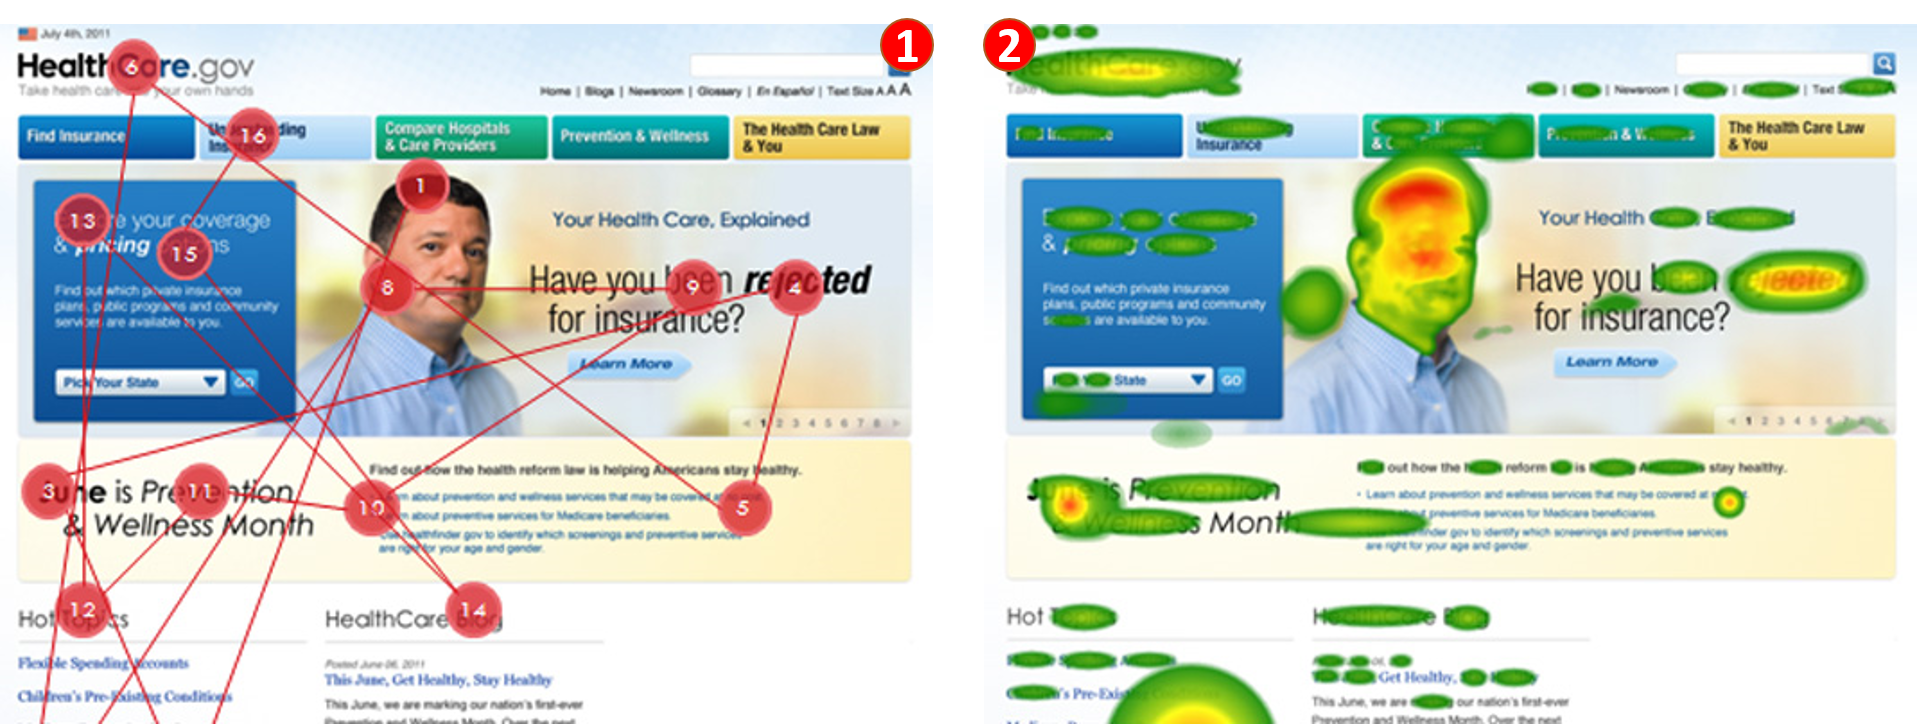
\includegraphics[width=1\linewidth]{img/Evaluation/Eyetracking}
\caption[Auswertungen der Eyetrackinganalyse]{Auswertungen der Eyetrackinganalyse. Linkes Bild (Marker 1): Ansicht einer ausgewerteten Blickabfolge. Rechtes Bild (Marker 2): Ansicht einer ausgewertet Heatmap (Quelle: https://www.usability.gov/how-to-and-tools/methods/eye-tracking.html - Stand Sommer 2016)}
\label{fig:Eyetracking}
\end{figure}


\subsubsection{Fragebogen}
\label{FragebogenEvaluation}


Während beim Eyetracking objektive Messungen  (Dauer des Ablaufs, Blickreihenfolge, etc.) durchgeführt werden stellt die Methode des Fragebogens eine Subjektive Messung da.
Da der Faktor Zufriedenheit in erste Linie subjektiv zu messen ist besteht ein Bedarf dies zu analysieren (vgl. \cite{Ollermann2007}, S. 57).
Zusätzlich besteht die Notwendigkeit, aus Sicht der Evaluierung, weitere Informationen (wie Beispielsweise Selbsteinschätzungen oder Anmerkungen zum Prototypen) ergänzend zum Eyetracking erheben (vgl. \cite{Laugwitz2006}, S. 127). \\
\\
Die Vorteile der Methode des Fragebogens liegen unter anderen in der guten Auswertbarkeit , speziell bei dem Einsatz von geschlossenen Fragen\footnote{Bei geschlossenen Fragen können die Proband\_innen ausschließlich auf vordefinierte Antworten zurückgreifen (vgl. \cite{Ollermann2007}, S. 61)}, der erhobenen Daten was auch der Grund für seine häufige Verwendung (vgl. \cite{Ollermann2007}, S. 61). 
Bei der Erstellung des Fragebogens darauf zu achten, das es sich nicht ausschließlich um eine Ansammlung von Fragen handelt.
Auf der anderen Seite gibt es auch Nachteile, welche unterstreichen das es sich um ein subjektives Verfahren handelt, wie Ollemannn in folgenden vier Punkten skizziert.
Bei dem Halo-Effekt liegt eine Tendenz nahe das die Beurteilung auf Grund eines Globalen Pauschalurteils (Beispielsweise die Farbgebung) gefällt wird.
Die Abgabe von systematisch zu positiven oder negativen Bewertungen (Milde-Härte-Fehler) oder das Gegenteil davon die Zentrale Tendenz bei dem Bewertungen im mittleren Bereich der Skala abgeben werden.
Abschließend führt er den Primacy-Recency-Effekt auf bei der die Bewertung durch die Reihenfolge der einzelnen Fragen beeinträchtigt wird. (siehe \cite{Ollermann2007}, S. 60)\\
\\
Damit der Fragebogen als funktionales Werkzeug bei der Evaluierung eingesetzt werden kann empfiehlt Burmester zusätzlich die Beachtung von Gütekriterien bei der Erstellung. 
Dabei handelt es sich sind unter anderen um das Gütekriterium der Validität\footnote{Der Fragebogen sollte darauf ausgelegt sein, dass zu messen was er vorgibt. (nach \cite{Burmester}, S. 350)}, - das Gütekriterium der Reliabilität\footnote{Ein wiederholtes Durchführen, unter den gleichen Bedingungen, soll zu dem selben Ergebnis führen. (nach \cite{Burmester}, S. 350)} und das Gütekriterium der Objektivität\footnote{Das Ergebnis ist unabhängig von der Person, welche die Untersuchung durchführt. (nach \cite{Burmester}, S. 350)}. \\



\subsection{Aufbau der Evaluation}
Anhand der Evaluation soll zum einen Untersucht ob der Prototyp den Anforderungen der Usability-Standards (Gebrauchstauglichkeit)\footnote{Gebrauchstauglichkeit nach ISO 9241 (\cite[siehe:][Abs.: 3.1 Gebrauchstauglichkeit]{Iso9241_11})} entspricht und zum anderen wie die Testpersonen die einzelnen Darstellungsformen der Daten (Karten- und Listenansicht) einsetzen und verwenden.
Dabei ist die Evaluation in die drei Teilbereiche Einführung, Eyetracking-Test und Fragebogen untergliedert.

\paragraph{Einführung}
Aufgrund des unterschiedlichen Wissensstände\footnote{Es wurden unter andern Personen ausgewählt die weder Erfahrung mit Pery haben und/oder in den Entstehungsprozess des Prototyps involviert waren.} der Testpersonen, ist es notwendig einen gemeinsamen Nenner zu bilden was mit Hilfe der Einführung realisiert werden soll.\\
\\
Im ersten Teil der Einführung werden Testpersonen denen Pery fremd ist die Hintergründe und der grobe Funktionsumfang von Pery erläutert.
Der zweite Teil beschäftigt sich damit den Testpersonen das Szenario zu erläutern. 
Dabei wird ihnen erklärt, das Sie im Außendienst tätig sind und anhand der gegeben Aufgabenstellung sowie mit Hilfe des Prototypen eine Menge an Partner Unternehmen für  Außendiensteinsätze auswählen sollen.
Im dritten Teil werden im groben die Funktion und die unterschiedlichen Bereiche des \ac{UI}'s vorgestellt. 
Diese Erläuterung wird ausschließlich mündlich und nicht am Prototypen durchgeführt um Platz für eigene Erkundungsversuche beim Test einzuräumen.
Abschließend wird die Aufgabenstellung für den Eyetracking-Test erläutert und eventuelle Unklarheiten beseitigt.


\paragraph{Eyetracking-Test}
Um ein möglichst realistisches Ergebnis der Testes für die Evaluation zu erhalten, orientiert sich der Aufbau weit möglichst an die realen Bedingungen welche im Abschnitt \nameref{Nutzungskontext} beschrieben werden.
Beispielsweise können Abweichung bei der Größe- und Auflösung des Monitors oder des Webbrowsers in dem der Prototyp verwendet wird zu unterschiedlichen Darstellungen führen. 
Dies kann wiederum dazu führen das weniger Informationen angezeigt werden wodurch die Effizienz eingeschränkt wird. (vgl. \cite{Ollermann2007}, S. 40)\\
\\
Für den Test wurde folgende Aufbau verwendet:
\begin{enumerate}
	\item Laptop mit installierter Tobii Software Suite\footnote{Wird verwendet um den Eyetracking Test aufzuzeichnen.}
	\item 24 Zoll Monitor mit einer Auflösung von 1920x1080 Pixel
	\item Mozilla Firefox Version: XXXX
	\item Webcam mit Mikrophon für die Aufzeichnung der Testperson während des Testes
\end{enumerate}

Der Test selbst ist in drei Stufen unterteilt, dabei wird bei jeder Stufe die Komplexität zum lösen der Aufgabe erhöht. 
In jedem der drei Problemstellungen ist die Testperson angehalten eine Außendiensteinsatz zu planen. 
Die jeweilige Schwierigkeit wird dabei durch die zusätzlichen Bedingungen definiert.
Anhand dieser Vorgehensweise soll anschließend ermittelt werden, wie sich die Bearbeitungsdauer, unter der Berücksichtigung des Erfahrungsgrades der Testperson, verhält. \\
\\
Als Referenzwert dient der erste Durchgang, hier soll ausschließlich ein Kontakt gefunden und ausgewählt werden. 
In der zweiten Aufgabe wird die Visualisierung von Informationen aus dem System benötigt. 
Dabei ist wiederum ein Kontakt, als primäres Ziel, gegeben die Testperson soll mithilfe des Prototypen und unter der Berücksichtigung von zwei Auswahlkriterium (letzte Rechnung vor dem 01.04.2016 und nicht weiter als 500 Meter Luftlinie vom primären Ziel entfernt) einen weiteren Kontakt (sekundäres Ziel) auswählen. 
Bei der dritten Aufgabe sollen drei Unternehmen auf dem Weg von A nach B ausgewählt werden.
Dabei ist der Start- sowie der Endpunkt definiert, die Route darf allerdings frei gewählt werden. 
Des weiteren sind die zusätzliche Auswahlkriterien letzter Besuch vor dem 01.05.2016 sowie Jahresumsatz von mehr als 10.000 Euro.
\\
Die Aufgabenstellung welches den Testpersonen ausgehändigt wird befindet sich im Anhang (siehe Abschnitt: \nameref{anhangEyetracking}).

\paragraph{Fragebogen}
Neben der Erfragung der subjektiven Meinung über das Produkt soll nach Ollermann auch Informationen über den Hintergrund der befragten Person erhoben werden.
Um diesen Hintergrund zu protokollieren empfiehlt er folgende Aspekte zu erheben Alter, Geschlecht und Erfahrung.
Speziell der Grad der Erfahrung stellt laut Ollermann einen "wesentlichen Einflussfaktor" für die Gebrauchstauglichkeit da. (vgl. \cite{Ollermann2007}, S. 46). 
Neben der eigentlichen Erfahrung mit dem Umgang von Pery, in welches der Prototyp eingebettet ist, stellt sich auch vergleichsweise die Frage ob und wie ausgeprägt Erfahrungen mit den Webservices vorhanden sind welche im Kapitel \nameref{chap:analyse} behandelt werden (siehe Abschnitt: \nameref{chap:analyse:sec:sota:sec:google_maps}, \nameref{Airbnb} und \nameref{Flightradar}).\\
\\
In erster Linie dient der Fragebogen, wie Eingangs erwähnt, als Unterstützung für die \nameref{Eyetracking}-Tests um eine subjektive Meinung bezüglich der drei Gebrauchstauglichkeits-Dimensionen zu erheben. 
Zum einen basiert der Fragebogen aus eigenen Fragen zum anderen in Anlehnung an standardisierten Fragebögen.
Von den standardisierten Fragebögen handelt es sich zum einen um den Fragebogen IsoMetric S (vgl. \cite{IsoMetricS}) und zum anderen um ISONORM (vgl. \cite{IsonormL}).
Da der ISONORM Fragebogen für die Analyse der Software Ergonomie-Norm (vgl. \cite{IsonormL}, S. 1) und nicht der Gebrauchstauglichkeit werden nur wenige Fragen erstellt die auf diesem Fragebogen basieren.
Im Gegensatz dazu, dient der IsoMetrics-Fragebogen als weitaus größere Kreativitätsquelle bei der Erstellung des Fragebogens.
Speziell die Möglichkeit, das Testpersonen sich bei Fragen ihrer Bewertung enthalten können wird als nützliches Element in die Befragung aufgenommen\footnote{Vorbeugung des Zentrale Tendenz-Problem welches zuvor in diesem Abschnitt beschrieben wurde.}\\
\\
Zusätzlich ist am Ende des Fragebogens/Interviews Platz für Anmerkungen vorgesehen welche während des Eyetrackings von den Testpersonen geäußert wurden.
An dieser Stelle soll mithilfe der entsprechenden Testperson geklärt werden wodurch diese Aussage provoziert wurde und ob sie negativ oder positiver Natur ist. (vgl. \cite{Niegemann2008}, S. 422)\\
\\
Der finale Fragebogen kann im Anhang (siehe Abschnitt: \nameref{anhangFragebogen}) eingesehen werden.

\subsection{Stichprobenbeschreibung}
\label{Stichproben}
In Summe wird die Evaluation mit elf Personen durchgeführt. 
Die Dauer der vollständige Evaluation liegt im mittleren Wert bei ca. 29 Minuten\footnote{Diese gesamt Dauer bezieht sich auf den Zeitraum der Einführung, des Eyetracking-Test und des Fragebogens}.
Dabei liegt der mittlere Wert des Alters bei 25,5 Jahren (min: 22 Jahren, max: 29 Jahren, einmal keine Angabe). 
Die elf Personen geben dabei folgende Nennungen beim Geschlecht an: dreimal männlich, sechsmal weiblich sowie zweimal kein Angabe.
Da der Prototyp als Erweiterung für Pery implementiert ist werden die Testpersonen, anhand Ihrer Erfahrungen im Umgang mit Pery, in drei Gruppen eingeteilt. 
Dabei werden die Gruppen wie folgt definiert: 
\begin{itemize}		
	\item Gruppe 1: keine Erfahrung mit Pery 
	\item Gruppe 2: geringe bis mittlere Erfahrung mit Pery
	\item Gruppe 3: ausgeprägte Erfahrung mit Pery
\end{itemize}
Die Zuordnung der Testpersonen zu denn entsprechenden Gruppen wird anhand der Faktoren der durchschnittliche Verwendung von Pery (in Stunden pro Woche) sowie der Dauer (in Monaten) seit dem Pery in Verwendung ist durchgeführt.
Anhand dieser Zuordnung stellt sich heraus das sechs Personen der Gruppe 1, drei Personen der Gruppe 2 und zwei Personen der Gruppe 3 zugeordnet werden. 


\section{Ergebnisse}
\label{Ergebnisse}
\ideas{nüchtern und ohne Interpretation}
Anhand der Evaluation soll zum einen Untersucht ob der Prototyp den Anforderungen der Usability-Standards (Gebrauchstauglichkeit)\footnote{Gebrauchstauglichkeit nach ISO 9241 (\cite[siehe:][Abs.: 3.1 Gebrauchstauglichkeit]{Iso9241_11})} entspricht und zum anderen wie die Testpersonen die einzelnen Darstellungsformen der Daten (Karten- und Listenansicht) einsetzen und verwenden. 
Um ein vermischen der Themen zu vermeiden werden die spezifischen Ergebnisse \nameref{ergebnis_usability} und \nameref{ergebnis_darstellungsformen} jeweils in einem separaten Absatz aufgezeigt.

\subsection{Usability Analyse}
\label{ergebnis_usability}
Für die Bewertung der Usability Analyse werden in erster Linie die Antworten aus dem Fragebogen herangezogen.
Im speziellen sind dabei die Antworten aus den drei Kategorien Effektivität (K\low{Effektivität}\footnote{K\low{Effektivität}: Kategorie Effektivität}), Effizienz (K\low{Effizienz}\footnote{K\low{Effizienz}: Kategorie Effizienz}) und Zufriedenheit (K\low{Zufriedenheit}\footnote{K\low{Zufriedenheit}: Kategorie Zufriedenheit}) von Interesse und werden hier folgt vorgestellt.
Bei allen drei Kategorien (K\low{Gesamt}\footnote{K\low{Gesamt}: Alle Kategorien}) wird dabei nach dem selben Schema vorgegangen. 
Die Fragen in den jeweiligen Abschnitten des Fragebogens konnten auf einer Skala mit den Werten 1 bis 5 beurteilt werden. 
Dabei bedeutet der Wert 5, dass die Testperson der Frage zustimmt und der Wert 1, dass Sie nicht zustimmt. 
Ein hoher Wert (Bsp.: 5) bedeutet dabei, das dass Anwendungserlebnis von der Testperson positiv in der entsprechenden Kategorie (K\low{Effektivität}, K\low{Effizienz} und K\low{Zufriedenheit}) war und ein niedriger Wert (Bsp.: 1) das es in der Kategorie negativ war.\\
\\
Für die Usability Analyse werden alle Antworten, welche einer Kategorie zu geordnet sind zusammengefasst und summiert. 
\textbf{Beispiel:} \\
Zur K\low{Effektivität} wurden fünf Fragen \footnote{Q\low{Effektivität}: Alle Fragen die K\low{Effektivität} zugeordnet sind.}) gestellt. 
Diese Fragen (Q\low{Effektivität}) wurden von einer Testperson mit den Werten 4,4,4,4,4 (5x 4) beantwortet (A\low{Effektivität}\footnote{A\low{Effektivität}: Alle Antworten die der Kategorie Effektivität (K\low{Effektivität}) zugeordnet werden.}), somit ist das Ergebnis, Summe der Punkten aus allen A\low{Effektivität} (R\low{Effektivität}\footnote{R\low{Effektivität}: Summe der Punkten aus allen A\low{Effektivität}}.) in dieser Kategorie 20 (R\low{Effektivität} = 20).\\
\\
Für jede K aus K\low{Gesamt} (Effektivität, Effizienz und Zufriedenheit) werden die drei Grenzen: Min. Grenze, Max. Grenze und 50\% Grenze separat definiert, da sie von der Anzahl der Fragen abhängig sind. 
Diese Grenzen dienen zum einen als Grundlage für die Bewertung der jeweiligen Kategorie (50\% Grenze) und zum anderen in der Visualisierung der Auswertungsdaten als Orientierungshilfen.
\paragraph{Min. Grenze} Der Wert für die Min. Grenze ist von der Anzahl Q\low{Kategorie} abhängig. Da jede Frage mit mindestens 1 Punkt beantwortet werden kann ergibt sich folgende Berechnung:\\
\\
Anzahl Q\low{Kategorie} x Min. Punkte = Anzahl Q\low{Kategorie} x 1 = Anzahl Q\low{Kategorie}
\paragraph{Max. Grenze} Der Wert der Max. Grenze ist ebenso wie der Wert der Min. Grenze von der Anzahl Q\low{Kategorie} abhängig. 
Da jede Frage mit bis zu 5 Punkten beantwortet werden kann ergibt sich folgende Berrechnung:\\
\\
Anzahl Q\low{Kategorie} x Max. Punkte = Anzahl Q\low{Kategorie} x 5 

\paragraph{50\% Grenze} Nur wenn R\low{Kategorie} (Ergebnisse)  über dieser Grenze liegen kann diese Kategorie als positiv gewertet werden.
Dabei verläuft die 50\% Grenze symmetrisch im Zahlenraum zwischen der Min.- und Max Grenze
Die Berechnung der 50\% Grenze ergibt sich daraus wie folgt:\\
\\
50\% Grenze = (Max. Grenze - Min. Grenze) / 2 + Min. Grenze\\
\\
Eine Ausnahme bildet die Kategorie Effektivität, diese kann nur als positiv gewertet werden wenn, zusätzlich zu den 50\%, auch jede Testperson die Aufgabenstellung korrekt bearbeitet hat.


\paragraph{Aufbau der Diagramme} \label{AufbauDiagramm} Um die Daten der Auswertung zu visualisieren wurde für jede Kategorie ein Diagramm angefertigt (siehe Abb.: \ref{fig:AuswertungEffektivitaet}, \ref{fig:AuswertungEffizienz} und \ref{fig:AuswertungZufriedenheit}), welches in dem jeweiligen Absatz zu finden ist.
Der Aufbau und die Gestaltung aller drei Diagramm sind dabei identisch und werden im folgenden erläutert.
Die Ergebnisse (R\low{Kategorie}) sind in vier Bereiche gruppiert, dabei stellt jeder Gruppierung eine definierte Testgruppe da. 
Zusätzlich zu den drei Testgruppen wurde eine Gruppierung über alle Datensätze (alle Testgruppen) erstellt (Im Diagramm mit Gesamt beschriftet). 
Jeder Gruppierung (Gruppe 1, -2, -3 und Gesamt) besteht dabei aus den drei Säulen mit der Beschriftung Min. Punkte (grüne Säule, links), Max. Punkte (blaue Säule, Mitte) und Mittelwert Punkte (helle Säule, rechts). 
Die definierten Grenzen Min. Grenze (schwarze Strich-Punkt Linie - vertikal), 50\% Grenze (rote Punkt Linie (vertikal)) und Max. Grenze (grüne Strich Linie - vertikal) wurden zum Zweck der Auswertung und Orientierung abgebildet.


\subsubsection{Effektivität}
Die Videoauswertung des Eyetrackings sowie die Analyse der Testdatenbank hat ergeben, das jede Testpersonen alle Aufgaben korrekt gelöst hat. 
Somit ist das erste Kriterium der Effektivität gegeben.\\
\\
Zu der Kategorie Effektivität wurden im Fragebogen fünf Fragen gestellt woraus sich folgende Grenzen definieren: Min. Grenze 5 Punkte, Max. Grenze 25 Punkte und 50\% Grenze 15 Punkte\\
\\
Anhand dieser Grenzen und den Werten aus R\low{Effektivität} wurde das Diagramm \nameref{fig:AuswertungEffektivitaet} (siehe Abb.: \ref{fig:AuswertungEffektivitaet}) erstellt\footnote{Details siehe Abschnitt: \nameref{AufbauDiagramm}}.\\
\\
Der niedrigste Wert von allen R\low{Effektivität} liegt bei 18 Punkten und der größte Wert bei 24 Punkten.
Im Mittel lag der R\low{Effektivität} in der Gruppe 1 bei ca. 23,17 Punkten (Min. 22 Punkte und Max. 24 Punkte), in der Gruppe 2 bei 21 Punkten (Min. 19 und Max. 23 ) und in der Gruppe 3 bei 19 Punkten (Min. 18 und Max. 20)\\
(siehe Abb.: \ref{fig:AuswertungEffektivitaet}).

\paragraph{Resultat Effektivität} Da Min. R\low{Effektivität} mit 18 Punkten über der 50\% Grenze mit 15 Punkten liegt, kann das Kriterium Effektivität positiv gewertet werden.


\begin{figure}[H]
\centering
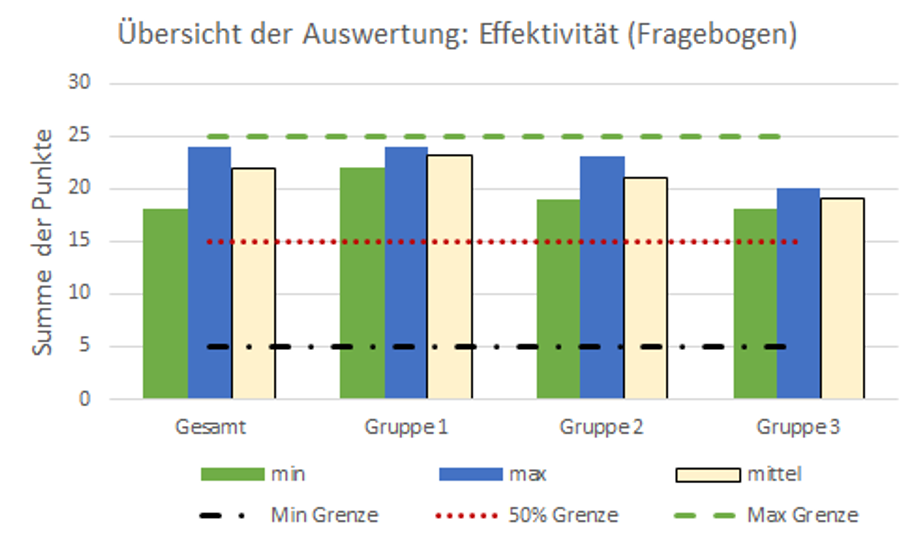
\includegraphics[width=0.9\linewidth]{img/Evaluation/Usability/AuswertungEffektivitaet}
\caption[Übersicht der Effektivität]{
	Auswertung Effektivität: Zeigt jeweils, nach Gruppen sortiert (siehe: \nameref{Stichproben}) sowie Gesamt (alle Gruppen), die summierten Punkte (Min. Punkte, Max. Punkte und Mittelwert Punkte) der Antworten aus dem Fragebogen, welche sich auf die Kategorie Effektivität beziehen. Quelle: eigene Ausarbeitung.
	}
\label{fig:AuswertungEffektivitaet}
\end{figure}


\subsubsection{Effizienz}
Zu der Kategorie Effizienz wurden im Fragebogen fünf Fragen gestellt woraus sich folgende Grenzen definieren: Min. Grenze 5 Punkte, Max. Grenze 25 Punkte und 50\% Grenze 15 Punkte\\
\\
Anhand dieser Grenzen und den Werten aus R\low{Effizienz} wurde das Diagramm \nameref{fig:AuswertungEffizienz} (siehe Abb.: \ref{fig:AuswertungEffizienz}) erstellt\footnote{Details siehe Abschnitt: \nameref{AufbauDiagramm}}.\\
\\
Der niedrigste Wert von allen R\low{Effizienz} liegt bei 20 Punkten und der größte Wert bei 25 Punkten.
Im Mittel lag der R\low{Effizienz} in der Gruppe 1 bei ca. 22,84 Punkten (Min. 21 Punkte und Max. 25 Punkte), in der Gruppe 2 bei ca. 22,67 Punkten (Min. 20 und Max. 25 ) und in der Gruppe 3 bei 22 Punkten (Min. 21 und Max. 23)\\
(siehe Abb.: \ref{fig:AuswertungEffizienz}).

\paragraph{Resultat Effizienz} Da Min. R\low{Effizienz} mit 20 Punkten über der 50\% Grenze mit 15 Punkten liegt, kann das Kriterium Effizienz positiv gewertet werden.

\begin{figure}[H]
\centering
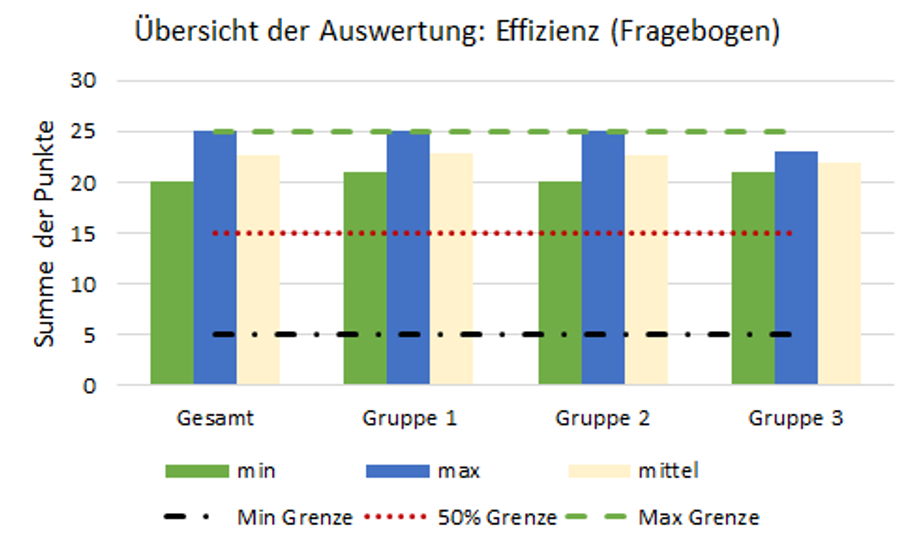
\includegraphics[width=0.9\linewidth]{img/Evaluation/Usability/AuswertungEffizienz}
\caption[Übersicht der Effizienz]{Auswertung Effizienz: Zeigt jeweils, nach Gruppen sortiert (siehe: \nameref{Stichproben}) sowie Gesamt (alle Gruppen), die summierten Punkte (Min. Punkte, Max. Punkte und Mittelwert Punkte) der Antworten aus dem Fragebogen, welche sich auf die Kategorie Effizienz beziehen. Quelle: eigene Ausarbeitung.}
\label{fig:AuswertungEffizienz}
\end{figure}


\subsubsection{Zufriedenheit}
Zu der Kategorie Zufriedenheit wurden im Fragebogen drei Fragen gestellt woraus sich folgende Grenzen definieren: Min. Grenze 3 Punkte, Max. Grenze 15 Punkte und 50\% Grenze 9 Punkte\\
\\
Anhand dieser Grenzen und den Werten aus R\low{Zufriedenheit} wurde das Diagramm \nameref{fig:AuswertungZufriedenheit} (siehe Abb.: \ref{fig:AuswertungZufriedenheit}) erstellt\footnote{Details siehe Abschnitt: \nameref{AufbauDiagramm}}.\\
\\
Der niedrigste Wert von allen R\low{Zufriedenheit} liegt bei 12 Punkten und der größte Wert bei 15 Punkten.
Im Mittel lag der R\low{Zufriedenheit} in der Gruppe 1 bei ca. 14,34 Punkten (Min. 13 Punkte und Max. 15 Punkte), in der Gruppe 2 bei ca. 13,67 Punkten (Min. 12 und Max. 15 ) und in der Gruppe 3 bei 14,5 Punkten (Min. 14 und Max. 15)\\
(siehe Abb.: \ref{fig:AuswertungZufriedenheit}).

\paragraph{Resultat Zufriedenheit} Da Min. R\low{Zufriedenheit} mit 12 Punkten über der 50\% Grenze mit 9 Punkten liegt, kann das Kriterium Zufriedenheit positiv gewertet werden.
\begin{figure}[H]
\centering
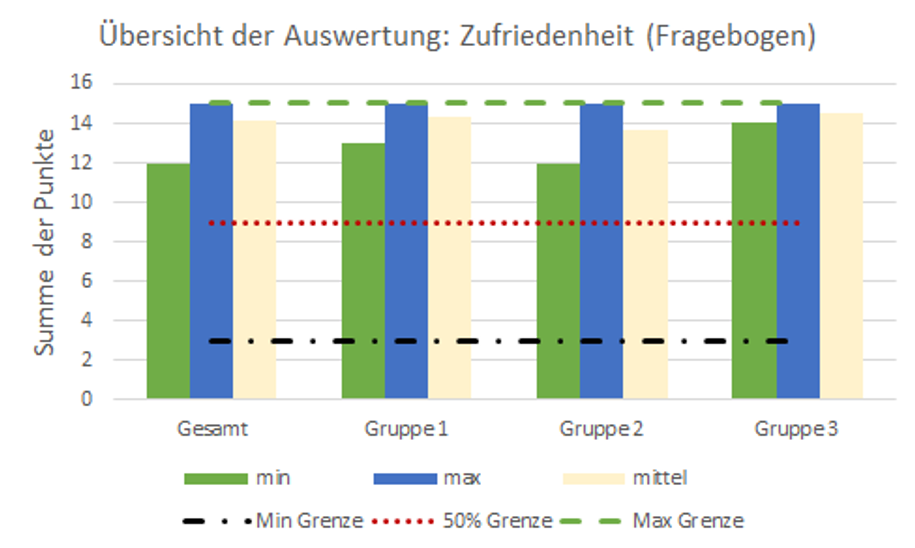
\includegraphics[width=0.9\linewidth]{img/Evaluation/Usability/AuswertungZufriedenheit}
\caption[Übersicht der Zufriedenheit]{Auswertung Zufriedenheit: Zeigt jeweils, nach Gruppen sortiert (siehe: \nameref{Stichproben}) sowie Gesamt (alle Gruppen), die summierten Punkte (Min. Punkte, Max. Punkte und Mittelwert Punkte) der Antworten aus dem Fragebogen, welche sich auf die Kategorie Zufriedenheit beziehen. Quelle: eigene Ausarbeitung.}
\label{fig:AuswertungZufriedenheit}
\end{figure}

\subsection{Eyetracking}
Anhand der dynamischen Webelemente (Karte zoomen und verschieben) konnten keine Gruppen basierte Analyse des Testes durchgeführt werden. 
Stattdessen wurden die Ergebnisse in erster Linie für die Analyse der \nameref{ergebnis_darstellungsformen} verwendet (siehe gleichnamigen Abschnitt). 

\subsection{Anmerkungen der Testpersonen}
\label{AnmerkungUser}
In diesem Abschnitt sollen die Anmerkungen der Testpersonen aufgezeigt werden. 
Während des Eyetracking-Testes wurden die Aussagen vom Testpersonal dokumentiert und im Anschluss des Fragebogens noch einmal mit den Testpersonen diskutiert.
Für einen besseren Überblick werden die jeweiligen Antworten, je nach Intention, in die Abschnitte positives Feedback sowie Optimierungspotential unterteilt. 

\paragraph{Positives Feedback}
10 von 11 Testpersonen haben sich während sowie nach dem Trip positiv zu der Unterstützung beim Planungsprozess geäußert. 
Davon haben zwei Testpersonen angegeben, das der Prototyp Alternativlos für das gegebene Testszenerio sei.  
Eine weitere Testperson gab an, das dass Maß an dargestellten Information optimal ausgewogen sei.

\paragraph{Optimierungspotential}
3 von 11 Testpersonen gaben an, das sie in der Listenansicht Probleme hatten, ein Unternehmen zur Auswahl hinzuzufügen.
Dabei versuchten Sie, das Unternehmen durch einen Klick auf den Namen, welcher als Link formatiert ist der zu Detailansicht des Kunden führt, zur Auswahl hinzuzufügen (siehe Abb.: \ref{fig:AddButton}).
Weitere fünf Testperson versuchten auf die gleiche Weise ein Unternehmen hinzuzufügen aber äußerten sich nicht während des Testes dazu.

\begin{figure}[H]
	\centering
	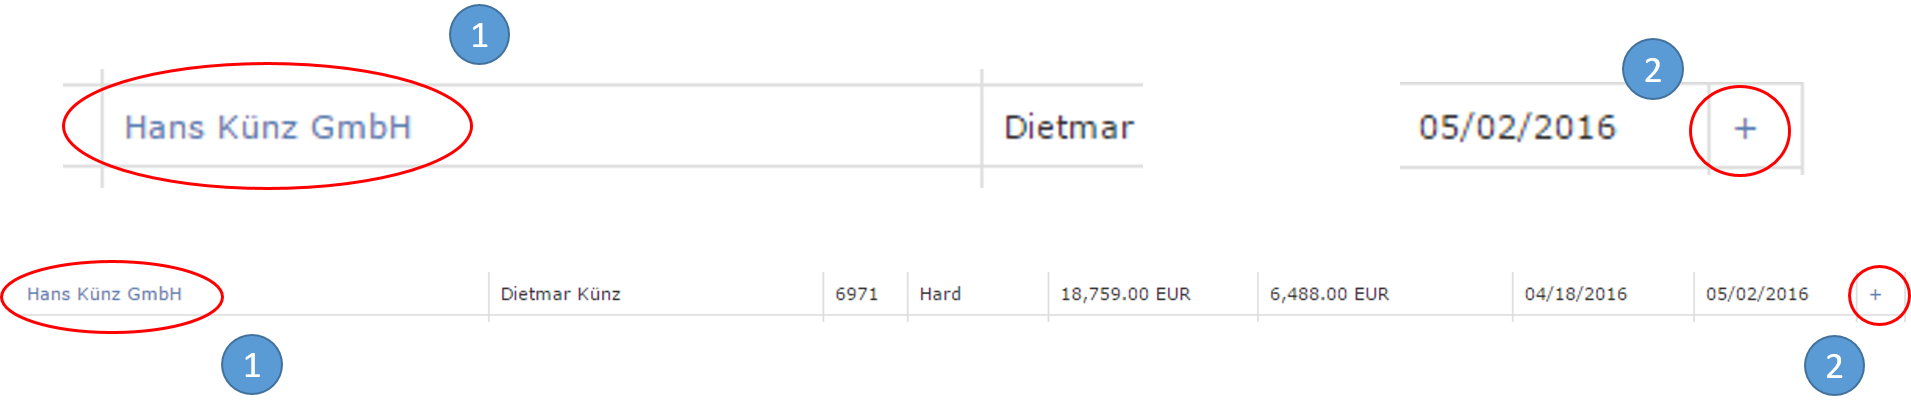
\includegraphics[width=1\linewidth]{img/Evaluation/Userfeedback/AddButton}
	\caption[Auschnitt Listenansicht]{Bildschirmfoto einer Zeile in der Listenansicht. Markierung 1: Name des Unternehmens als Link zur Detailansicht des entsprechenden Unternehmens. Markierung 2: Button mit der Beschriftung Plus (+) um das Unternehmen zur Auswahl hinzuzufügen. Sämtliche Zahlen sind fiktiv. Quelle: eigene Ausarbeitung.}
	\label{fig:AddButton}
\end{figure}
Da der Prototyp, laut Definition, mit englischer Benutzeroberfläche implementiert wurde weicht das Datumsformat dementsprechend von dem deutschen Datumsformat ab. 
Für 3 von 11 Testperson war das englische Datumsformat (Monat/Tag/Jahr) so irritierend das es es während des Testes angesprochen wurde.

\subsection{Verwendung und Einsatz der Darstellungsformen}
\label{ergebnis_darstellungsformen}
Für die Auswertungen der verwendeten Darstellungsformen dient in erster Linie die Videomitschnitte des Eyetracking Tests. 
Dabei bearbeiteten die Testpersonen jeweils drei verschiedene Aufgabenstellungen welche ein ansteigendes Komplexitätsniveau aufweisen.
Im folgenden Text werden die einzelnen Aufgabenstellungen als Trip bezeichnet.
\footnote{Eine Übersicht über die Aufgabenstellung des Eyetrackingtests findet sich im Abschnitt \ref{Verfahren} - \nameref{Verfahren}. Der vollständige Test befindet sich im Anhang (siehe Abschnitt \ref{anhangEyetracking} - \nameref{anhangEyetracking}). 
	}\\
	\\
Im ersten Schritt wurden, mit Hilfe des Eyetrackings, die Bearbeitungsdauern der einzelnen Trips pro Testperson ausgewertet und nach den entsprechenden Testgruppen gruppiert (siehe Abb.: \ref{fig:BearbeitungsdauerTrip}).  
Anhand dieser Datensätze wurde im ersten Schritt ausgewertet wie viel Zeit die einzelnen Testgruppen für die jeweiligen Trips benötigt haben.
Im Mittelwert lag die Bearbeitungsdauer für Trip 1 zwischen 54 Sekunden und 02:35 Minuten, für Trip 2 zwischen 01:20 Minuten und 03:09 Minuten sowie für Trip 3 zwischen 03:06 Minuten und 04:39 Minuten (siehe Abb.: \ref{fig:BearbeitungsdauerTrip}).
\begin{figure}[H]
\centering
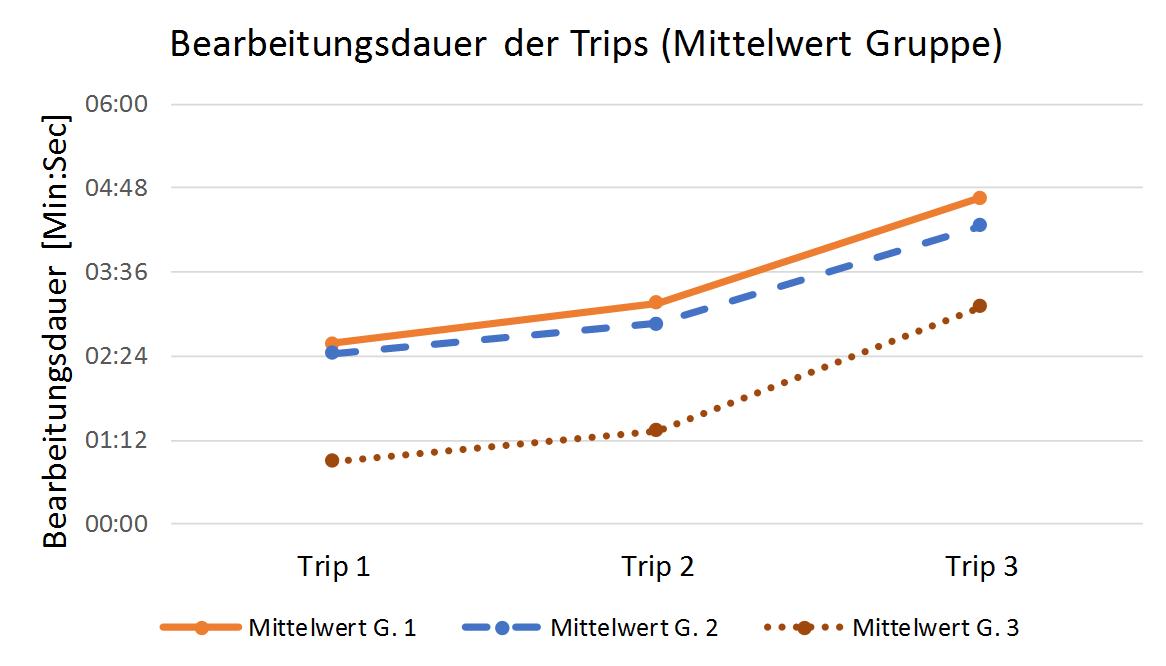
\includegraphics[width=0.7\linewidth]{img/Evaluation/Darstellungsformen/BearbeitungsdauerTrip}
\caption[Übersicht der Bearbeitungsdauer]{Übersicht der Bearbeitungsdauer der einzelnen Trips in Minuten. Die Daten entsprechen dem Mittelwert der jeweiligen Gruppen.  
Quelle: eigene Ausarbeitung.
	}
\label{fig:BearbeitungsdauerTrip}
\end{figure}

Um die Art und Weise besser zu verstehen, wie die Testpersonen die jeweiligen Darstellungsformen bei der Planung der Trips verwendet haben, wurden im nächsten Schritt die Datensätze welche sich auf die der Darstellungsarten beziehen untersucht. 
Im ersten Schritt wurde dabei analysiert wie viel Zeit alle Gruppen (Summe) in den unterschiedlichen Ansichten verbracht haben (siehe Abb.: \ref{fig:VerwendungsdauerTrip}).
Um einen genaueren Einblick in die die Verwendungsdauer zu erhalten wurden daraufhin die Daten nach den Testgruppen aufgeschlüsselt (siehe Abb.: \ref{fig:VerwendungsdauerGruppe}).
Ergänzend zu dem Aspekt der Zeit wurden zusätzlich die Wechsel zwischen den Ansichten ausgewertet. 
Das Diagramm beschreibt wie oft innerhalb einer Gruppe eine Testperson (Mittelwert der Gruppe) die jeweilige Ansicht in den unterschiedlichen Trips aufgerufen hat (siehe Abb.: \ref{fig:Haufigkeit}). 


\begin{figure}[H]
\centering
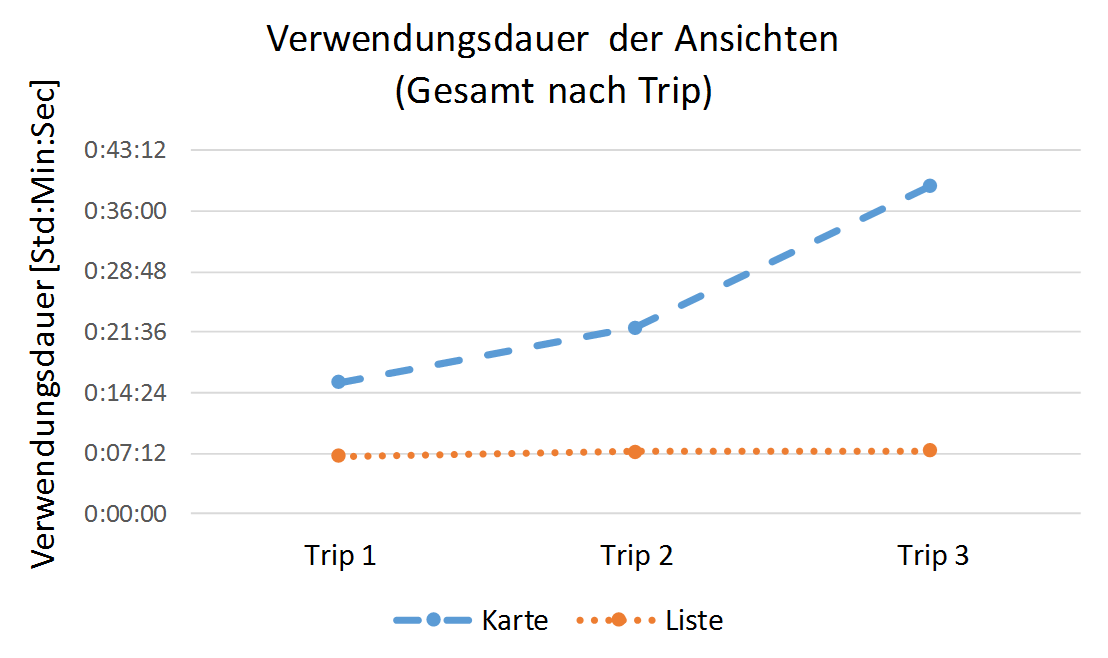
\includegraphics[width=0.7\linewidth]{img/Evaluation/Darstellungsformen/VerwendungsdauerTrip}
\caption[Verwendungsdauer der verschiedenen Ansichten.]{Übersicht über die Verwendungsdauer der verschiedenen Ansichten. Die Daten beziehen sich auf alle Gruppen (Summe) und wurden nach Trip gruppiert. Quelle: eigene Ausarbeitung.}
\label{fig:VerwendungsdauerTrip}
\end{figure}

\begin{figure}[H]
\centering
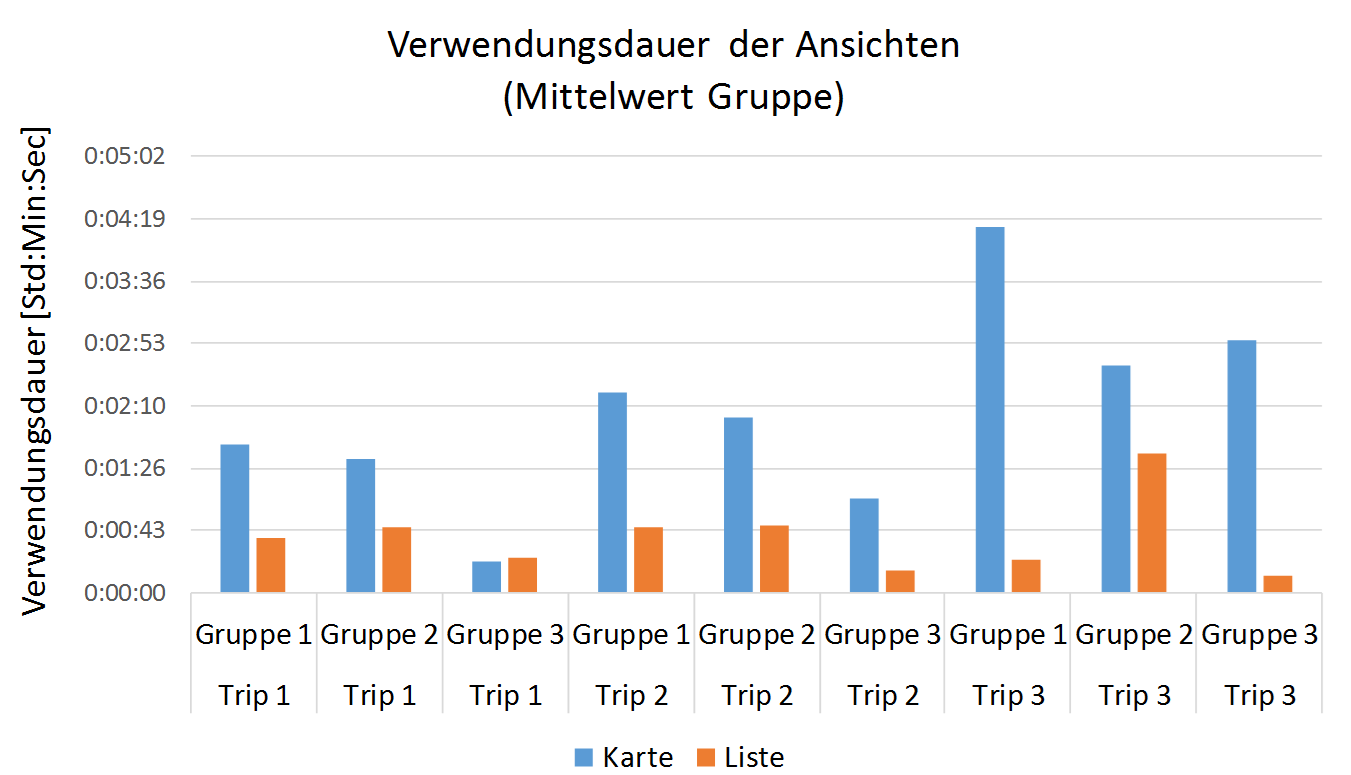
\includegraphics[width=0.7\linewidth]{img/Evaluation/Darstellungsformen/VerwendungsdauerGruppe}
\caption[Übersicht Verwendungsdauer Ansichten (Detail)]{Verwendungsdauer der verschiedenen Ansichten im Detail. Es wurden die Daten sowohl nach Gruppe (Mittelwert der Gruppe) als auch nach Trip gruppiert. Quelle: eigene Ausarbeitung.}
\label{fig:VerwendungsdauerGruppe}
\end{figure}

\begin{figure}[H]
\centering
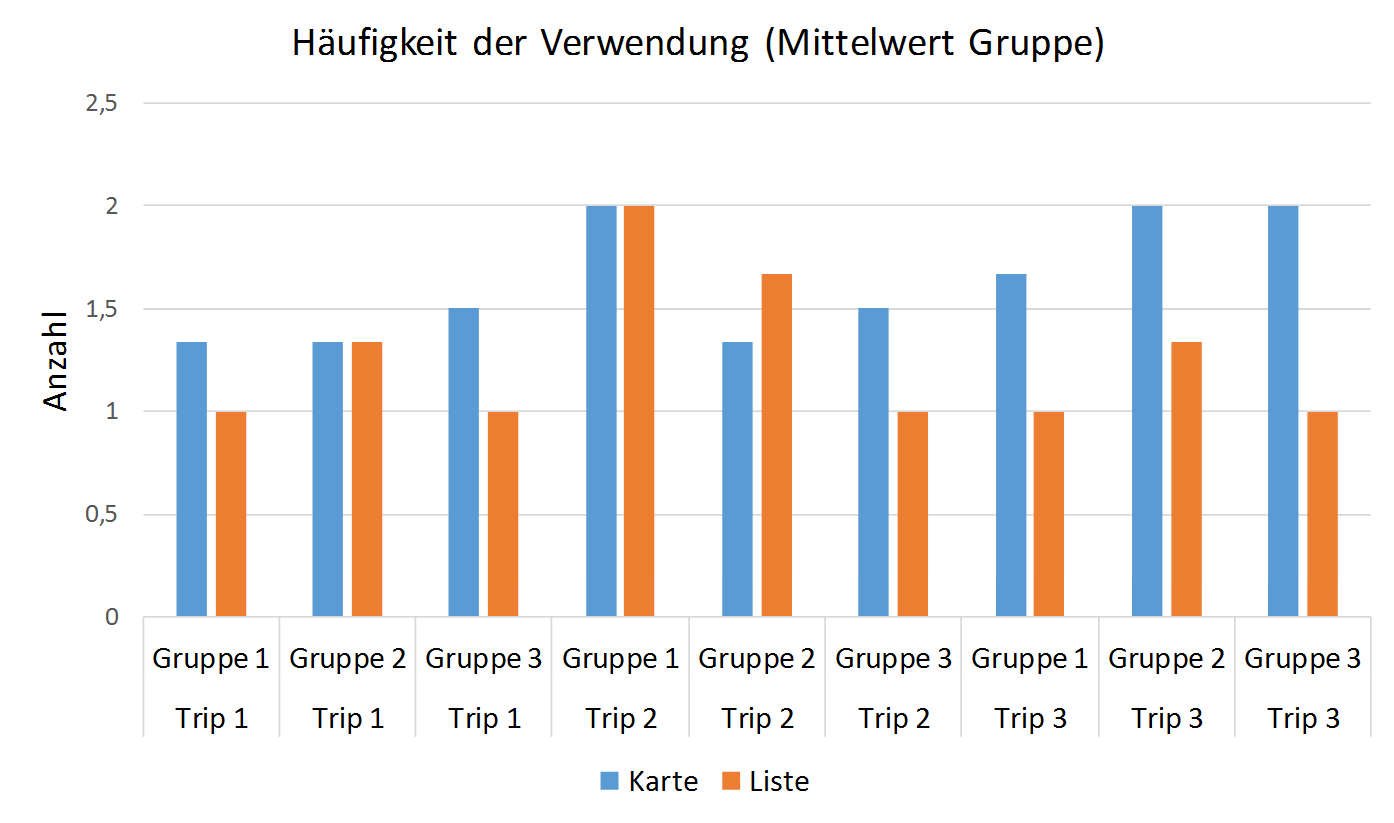
\includegraphics[width=0.7\linewidth]{img/Evaluation/Darstellungsformen/Haufigkeit}
\caption[Häufigkeit der der verwendeten Ansichten]{Übersicht über die Häufigkeit der Aufrufe der verschiedenen Ansichten. Das Diagramm zeigt an wie oft die jeweilige Ansicht in dem entsprechenden Trip aufgerufen wurde. Die Daten sind nach dem Mittelwert der Gruppe sowie nach Trip gruppiert. Quelle: eigene Ausarbeitung.}
\label{fig:Haufigkeit}
\end{figure}

\subsubsection{Meilensteine}
\label{Meilensteine} 
Für den letzten Schritt der Auswertung wurde für jeden Trip eigene Meilensteine definiert. 
Die einzelnen Meilensteine kennzeichnen einen Teilerfolg innerhalb eines Trips (Erste Ziffer: zugehöriger Trip, zweite Ziffer: aufsteigende Nummerierung) und wurden wie folgt definiert. 
\begin{itemize}
	\item Trip 1
	\item[] M1-1: Auswahl des genannten Kontaktes 
	\item Trip 2
	\item[] M2-1: Auswahl des genannten Kontaktes
	\item[] M2-2: Auswahl des gesuchten Kontaktes
	\item Trip 3
	\item[] M3-1: Auswahl des genannten Kontaktes
	\item[] M3-2: Auswahl des ersten gesuchten Kontaktes
	\item[] M3-3: Auswahl des zweiten gesuchten Kontaktes
	\item[] M3-4: Auswahl des dritten gesuchten Kontaktes
\end{itemize}
Anhand des Videomaterials des Eyetrackings wurde untersucht, welche Ansicht beim erreichen des jeweiligen Meilensteins von den Testpersonen verwendet wurde. 
Um die Ergebnisse dieser Auswertung zu visualisieren wurde Diagramm \ref{fig:Meilenstein} angefertigt. 
Für diesen Zweck wurden die ausgewerteten Daten nach Gruppe (Mittelwert) und Meilenstein gruppiert.
Dabei ist zu beachten, das die Daten in der Y-Achse gestapelt abgebildet wurden und der Wert 1 auf der Y-Skala 100\% entspricht. 

\begin{figure}[h]
\centering
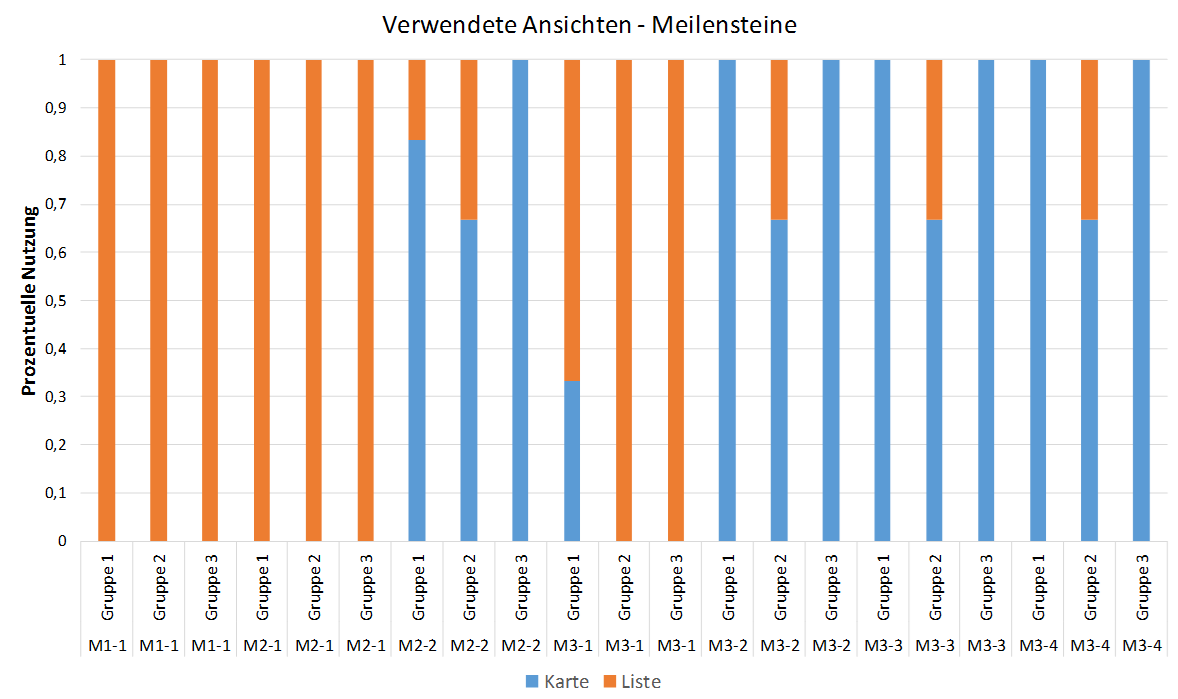
\includegraphics[width=1\linewidth]{img/Evaluation/Meilenstein}
\caption[Verwendete Ansichten - Meilensteine]{
	Übersicht über die verwendeten Ansichten beim erreichen des jeweiligen Meilensteins. Die Daten sind Mittelwerte über die jeweiligen Testgruppen und nach Meilensteinen sortiert (siehe Abschnitt \nameref{Meilensteine} für weitere Details). Y-Achse: die Daten werden gestapelt dargestellt, der Wert 1 entspricht 100\%.
	Quelle: eigene Ausarbeitung
	}
\label{fig:Meilenstein}
\end{figure}



\section{Interpretation \& Diskussion}
\label{InterpretationDiskussion}
Nachdem im letzten Unterkapitel die Ergebnisse des Testes präsentiert wurden, sollen an dieser Stelle mögliche Interpretationen dieser Informationen Besprochen werden.

\subsection{Usability Analyse}
Wie in dem entsprechenden Abschnitt schon dargelegt wurde, erreichten alle drei Kategorien einen positives Ergebnis. 
Somit kann gesagt werden das die Usability (im Rahmen der Definition Gebrauchstauglichkeit) gegeben ist. 
Bei der Auswertung der Fragebögen ist aufgefallen das bei zwei Fragen der Mittelwert der Antworten unter 4 von 5 Punkten liegt. 
Dies ist zum einen der Irritation der Testpersonen beim hinzufügen von Unternehmen zur Auswahl in der Listenansicht (Mittelwert ca. 3,9 von 5 Punkten) und zum anderen dem ungewohnten englischen Datumsformat (Mittelwert ca. 3,82 von 5 Punkten) geschuldet.
Diese beiden Punkte werden unter anderem im nächstem Abschnitt genauer betrachtet.\\
\\
Anhand der Testergebnisse, in dennen alle drei Kategorien als positiv definiert wurden kann die Hypothese als bestätigt angesehen werden.  

\subsection{Anmerkungen der Testpersonen}
Bei der Analyse sind die drei Themen Hinzufügen von Unternehmen in der Listenansicht, englisches Datumsformat sowie der Wunsch nach einer Filterfunktion am deutlichsten hervorgetreten.\\

\subsubsection*{Hinzufügen in der Listenansicht}
\paragraph{Beschreibung}
Innerhalb der Listenansicht, trat immer wieder bei den verschiedenen Testpersonen Verwirrung auf als sie sich unerwarteter Weiße in der Detailansicht des Unternehmen wiederfanden und nicht wie vermutet das entsprechende Unternehmen zur Auswahl hinzugefügt würde.

\paragraph{Hintergrund}
Dieses Erwartungshaltung ist vermutlich dem Umstand geschuldet, das die betroffenen Testpersonen in ihrem geistigen Modell die Funktion des Hinzufügens mit dem exponiert stehenden (links in der Zeile), als Link formatierten, Unternehmensnamen assoziieren. \\
\\
Um dies besser zu verstehen sollte der Aufbau der Listenansicht, im speziellen die Anordnung der Elemente in einer Zeile\footnote
{
	Anmerkung: Jede Zeile bildet in der Listenansicht ein Unternehmen ab.
	}
, betrachtet werden.
Bei der Erstellung des Konzeptes wurde entschieden nur die notwendigen Informationen abzubilden. Aus dieser Motivation heraus wurde der Name des Unternehmens, in beiden Ansichten, als Link gestaltet (siehe Abbildung: \ref{fig:AddButton} - Markierung 1) welcher die Detailansicht aufruft, falls weitere Informationen zu dem entsprechenden Unternehmen gewünscht werden.
\ideas{Zitat aus Usability Guideline raussuchen}
Desweiteren wurde, aus gründen der Konsistenz (vgl. \cite[S. 103, 11:4 Ensure Visual Consistency]{Koyani2004}), in der Listenansicht der eigentliche Button zum hinzufügen im rechten Bereich der Zeile, innerhalb der Listenansicht, platziert (siehe Abbildung \ref{fig:AddButton} - Markierung 2). 
\footnote{
	Innerhalb von Pery sind Funktionen welche sich auf Zeilen in Listen beziehen (bearbeiten, löschen, etc.) rechts platziert.
	} 
und mit einem Plus (+) beschriftet wie auch im Popup der Kartenansicht (siehe Abbildung: \ref{fig:Add}).\\
\\
Folgende Begründungen könnten die Ursache dafür sein das die Testpersonen den Link des Unternehmensnamens verwendet haben und nicht den bereitgestellten Button.
Erstens könnte die Ursache in der Positionierung liegen. 
Der Hinzufüge Button ist zwar nicht außerhalb des Sichtfeldes gelegen allerdings ist der Unternehmensname, mit der Positionierung als zweites Element von links, deutlich hervorstechender.
Ein weiterer interessanter Fakt liegt darin das sich selbst versierte Pery-Nutzer\_innen beim ersten mal ähnlich verhalten haben. 
Ein weiterer Grund könnte darin liegen, das die Testpersonen durch das erlernte Verhalten im Umgang mit Webseiten daran gewöhnt sind das ein Link (Unternehmensname) eine Funktion, im Normalfall eine Weiterleitung, ausführt.
Zusätzlich ergaben die Gespräche mit den betroffenen Personen zum einen das der Button nicht als Markant genug wahrgenommen wurde und zum anderen das sie sich nicht im klaren waren über die Funktion. 
Allerdings war allen Testpersonen der Verwendungszweck des Buttons innerhalb Kartenansicht sofort verständlich.\\
\\
Mögliche Optimierungsvorschläge könnten unter anderem eine Änderung der Position und/oder die Änderung der Beschriftung in Hinzufügen wodurch zum einen mehr Aufmerksamkeit auf den Button gelenkt wird als auch das die Bedeutung klarer wird.

\begin{figure}[h]
	\centering
	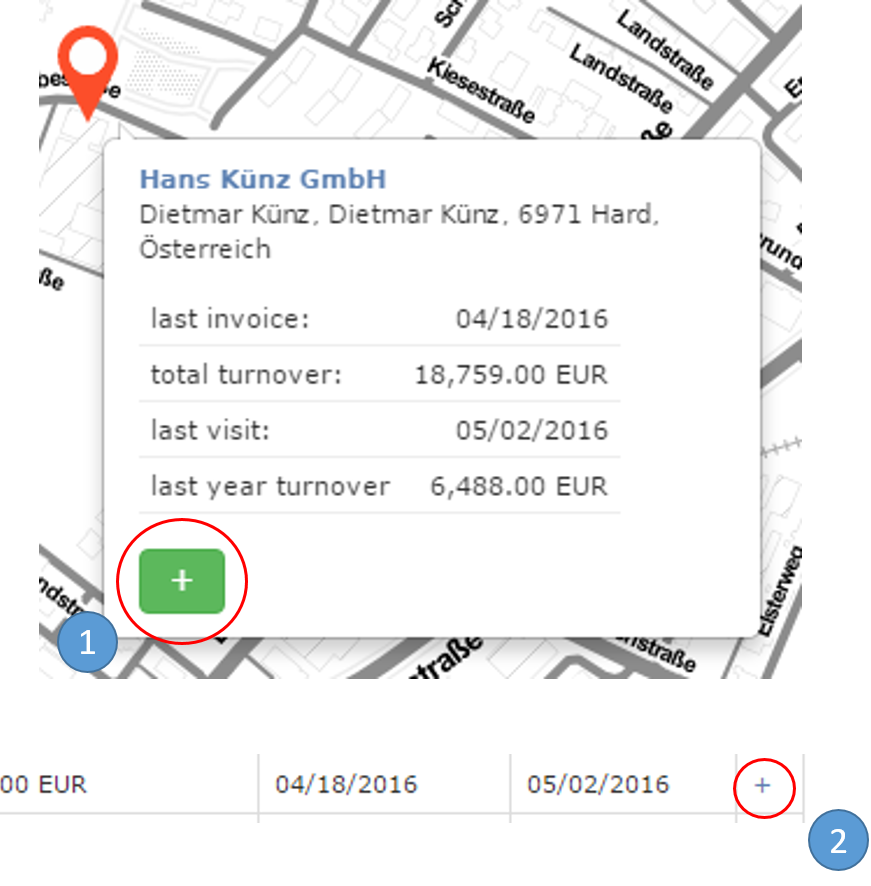
\includegraphics[width=0.7\linewidth]{img/Evaluation/Userfeedback/Add}
	\caption[Vergleich: Button Karte- und Listenansicht]{Vergleich Hinzufügen von Unternehmen (Button). Markierung 1: Button im Popup der Kartenansicht, Markierung 2: Button in der Listenansicht. Die angegebenen Daten auf der Abbildung sind fiktiv. Quelle: eigene Ausarbeitung.}
	\label{fig:Add}
\end{figure}

\subsubsection*{Datumsformat}
Da die gesamte Benutzeroberfläche in Englisch gehalten ist war das Datumsformat dementsprechend auch in Englisch gehalten. 
Für das Datumsformat wurde die Konstellation Monat/Tag/Jahr in Ziffern gewählt. 
Dies hat teilweise die Testpersonen in einem solchen Ausmaß irritiert das dabei merkbar die Effizienz gelitten hat da Sie jedes mal geistig das gegebene Datum in das verwendete Datumsformat des Prototypen übertragen mussten und umgekehrt.\\
\\
Als möglicher Optimierungsansatz könnten die Ziffern des Monatsformates durch eine Abkürzung des Monatsnamens ersetzt werden wie Beispielsweise: Oct. 10, 2016 wodurch das verwechseln der Monats- und Tagesziffer ausgeschlossen wird.  

\subsubsection*{Filterfunktion}
Um einen besseren Überblick bei der Planung zu erhalten gaben 3 von 11 Personen an, das sie gerne eine Filterfunktion verwenden würden.  
Diese Filterfunktion wurde zum einen für die Karten- als auch für die Listenansicht gewünscht.
Innerhalb der Kartenansicht sollen dabei Marker- und in der Listenansicht dementsprechend Zeilen ausgeblendet werden.
 

\subsection{Verwendung und Einsatz der Darstellungsformen}
Die Kombination der unterschiedlichen Datenvisualisierungen (Karten- und Listenansicht) in Verbindung mit der Anreicherung der Kerndaten mit den kontextsensitiven Daten ist von den Testpersonen sehr gut angenommen und im Fragebogen bekundet wurden (siehe Abschnitt: \nameref{Ergebnisse}).
Im speziellen beschäftigt sich dieser Abschnitt damit ob die gemessen Werte des Eyetracking Testes zu ähnlichen Ergebnissen kommen wie die subjektive Bewertung der Testpersonen.\\
\\
Als erster Schritt soll im Vorfeld die Bearbeitungsdauer der einzelnen Trips betrachtet werden da sie als Grundlage für die weiteren Annahmen dient. 
Dabei ist zu erkennen das die mittlerer Bearbeitungsdauer der Testpersonen nach einem ähnlichen Muster anwächst (siehe Abb. \ref{fig:BearbeitungsdauerTrip}).
Zusätzlich fällt dabei auf das, sich möglicherweise der Erfahrungswert im Umgang mit Pery auf die Bearbeitungsdauer niederschlägt.
Dieser Verdacht entsteht durch die Annahme, das die Gruppe mit der meisten Erfahrung in Pery (Gruppe 3) am schnellsten die Aufgaben abarbeitete gefolgt von der Gruppe mit mittleren Erfahrungsgrad (Gruppe 2) und zuletzt die Gruppe ohne Erfahrungen (Gruppe 3) im Umgang mit Pery (siehe Abb. \ref{fig:BearbeitungsdauerTrip}).
Dabei ist zu beachten das es sich hierbei ausschließlich um einen Verdacht handelt für eine Bestätigung müssten allerdings weitere Tests durchgeführt werden.\\
\\
Beginnend mit der Auswertung der absoluten Verwendungsdauer ist zu erkennen (siehe Abb. \ref{fig:VerwendungsdauerTrip}) das sich die Verwendungsdauer (Mittelwert aller Testpersonen) der Kartenansicht\footnote{Verwendungsdauer der Kartenansicht Trip 1: ca. 15 min., Trip 2: ca. 22 min. und Trip 3: ca. 39 min.} im Gegensatz zur Listenansicht\footnote{Verwendungsdauer der Listenansicht: zwischen 6:48 min. und 7:31 min.} stetig ansteigt.  
Im Detail werden die gleichen Daten nach Testgruppen gruppiert in Abbildung \ref{fig:VerwendungsdauerGruppe} dargestellt. 
Darauf lässt sich erkennen das bis auf eine Ausnahme die Testgruppen mehr Zeit in der Kartenansicht als in der Listenansicht zum lösen der Aufgabenstellung verbracht haben. 
Die Ausnahme stellt dabei die Gruppe 2 in Trip 1 da, was die einzige Situation ist, in der der Mittelwert einer Gruppe in der Listenansicht höher ist als in der Kartenansicht (Kartenansicht: 22 Sec. und Listenansicht 23 Sec.).
Diese Daten können wie folgt interpretiert werden: Mit dem ansteigen der Komplexität (siehe Abb. \ref{fig:VerwendungsdauerTrip}), steigt gleichzeitig die Nutzungsdauer der Kartenansicht in einem ähnlichen Muster (siehe Abb. \ref{fig:VerwendungsdauerGruppe}).\\
\\
Ergänzend zu der Dauer soll noch die Anzahl der Wechsel zwischen den einzelne Ansichten betrachtet werden (siehe Abb. \ref{fig:Haufigkeit}).
Dabei fällt auf das alle Gruppen sowohl die Karten- als auch die Listenansicht zum lösen der Aufgabenstellung verwendeten. 
Speziell in Trip 3 wurde allerdings am häufigsten zu der Kartenansicht gewechselt. \\
\\
Zusätzlich zu den einzelnen Trips wurden Meilensteine definiert welche Teilerfolge innerhalb der Trips darstellen.
\footnote{
	Die Definition der einzelnen Meilensteine können im gleichnamigen Abschnitt der Sektion \nameref{Ergebnisse} nachgeschlagen werden.
	}
Anhand der Auswertungen ist ersichtlich welcher Meilenstein mit welcher Ansicht erreicht wurde (siehe Abb. \ref{fig:Meilenstein}). 
Dabei ist zu beachten das hierbei nur die Ansicht genannt wird, welche zum Zeitpunkt des Erreichens aktiv war und nicht welche Ansichten wie lange davor verwendet wurden um diesen Meilenstein zu erreichen.
Dabei lässt sich erkennen das in allen Meilensteinen in denen nur ein Wert gesucht wurde (Unternehmensname oder Gesamtumsatz) bei allen Gruppen der Einsatz der Listenansicht zum lösen des Meilensteins überwiegt. (siehe Abb. \ref{fig:Meilenstein} - Meilenstein: M1-1, M2-1 und M3-1).
Dementsprechend steigt der Anteil Kartenansicht zum lösen der komplexeren Meilensteine deutlich an (siehe Abb. \ref{fig:Meilenstein} - Meilenstein:  M2-2 und M3-2 bis M3-4).  \\
\\
Abschließend lässt sich zu der Auswertung der unterschiedlichen Darstellungsformen folgende Erkenntnisse zusammenfassen: 
\begin{itemize}
	\item[] Die Verwendung der jeweiligen Ansicht ist an die Komplexität bzw. die Art der  Aufgabenstellung gebunden.
	\item[] Bei Aufgabenstellungen mit einer Bedingung (siehe Trip 1 sowie erster Teil von Trip 2 und Trip 3) wurde bevorzugt die Listenansicht gewählt.
	\item[] Bei Aufgabenstellungen mit mehreren Bedingungen und/oder geografischen Abhängigkeiten (siehe zweiter Teil von Trip 2 und Trip 3) wurde bevorzugt die Kartenansicht eingesetzt. 
\end{itemize}
Somit lässt sich Schlussendlich sagen das die Kartenansicht zwar die konservative Listenansicht sinnvoll ergänzt allerdings nicht, in der Form dieses Prototypen, ersetzt.



\end{document}